\newpage
\fancyhead[C]{Jihwan Shin}
\section{Extra-UAV Communication Architecture} \label{sec:euc}

Most of the procedures required in our system are processed offline either within the drone's internal hardware (e.g. control system, emergency protocol, data collection) or the base station computer (e.g. data processing, mission planning). However, it is necessary to enable an online communication system that can be used to send/receive necessary information between the drones and the base station during flight time. In this section, we outline the requirements of the extra-\gls{UAV} communication system and explore the use of \gls{lora} communication as the solution. A ns-3 simulation for \gls{lora} communication is also considered for integration with the mission planning framework. 

%%%%%%%%%%
\subsection{System Requirements}
\label{sec:euc_requirements}

\subsubsection{Base Station}

The base station is the central node where the drones are deployed to the \gls{roi}. It comprises of the main computer and a charging station for the drones. Its role throughout the mission is as follows:

\begin{itemize}
    \item \textbf{Before mission}: The main computer processes the mission planning framework to generate the path plan for each drone. The path is uploaded to the drones for them to follow offline during the mission. Drones are charged at the charging station to achieve the maximum travel distance possible. 
    \item \textbf{During mission}: The drones are in flight, following the offline path plan to collect the data with their thermal or \gls{GPR} sensors. The main computer receives the \gls{GNSS} data from all drones to keep track of their locations, and transmits emergency flags in case an extreme event forces the mission to be paused (e.g. rainfall, strong wind forecasts). They also calculate and communicate the necessary data for the \gls{RTS} algorithms explained in Section~\ref{sub_section:tgt_path_planning}. This is where the extra-\gls{UAV} communication becomes necessary. 
    \item \textbf{After mission}: The drones have returned to the base station and they are charged at the charging station. The data collected from the mission is uploaded to the main computer for processing to predict the location of the landmines. 
\end{itemize}

\subsubsection{Extra-UAV Communication Content}

Table~\ref{tab:euc_messages} lists all messages that should be communicated between the drones and the base station with details on content, direction and size. Each drone will be equipped with a transceiver that communicates with the base station's transceiver. Drone to drone communication is not established. 

\begin{table}[h]
    \centering
    \begin{tabularx}{\textwidth}{|>{\raggedright\arraybackslash}p{2.5cm}|X|>{\centering\arraybackslash}p{2.5cm}|>{\centering\arraybackslash}p{1.8cm}|}
        \hline 
        \centering{\textbf{Message}} & \centering{\textbf{Detail}} & \textbf{Direction (Drone-Base)} & \textbf{Size (bits)} \\ 
        \hline\hline
        Timestamp & Time data for confirmation of transmission period. & $\leftrightarrow$ & 64 \\
        \hline
        Drone ID & Distinct ID given to each drone to distinguish at the base station. Unsigned char (0-255) is used. & $\leftrightarrow$ & 8 \\
        \hline
        \gls{GNSS} Location & The x, y, z location coordinates of the drone based on \gls{GNSS}. Each dimension is expressed as a double (64-bits). & $\rightarrow$ & 192 \\
        \hline
        \gls{GNSS} \gls{RTK} Correction & Correction data required to achieve \gls{RTK} explained in Section~\ref{sub_sub_section:tgt_component_selection}.  The message size is estimated based on \cite{RTK_LORA}. & $\rightarrow$ & 500 \\
        \hline
        Controller ID & Data required for the \gls{RTS} system in Section \ref{sub_section:tgt_path_planning}. Unsigned char (0-255) is used. & $\rightarrow$ & 8 \\
        \hline
        $p$ & Data required for the \gls{RTS} system in Section \ref{sub_section:tgt_path_planning}. Unsigned integer (0-65535) is used which is scaled to a value between 0 and 1. & $\leftarrow$ & 16 \\
        \hline
        Return to Safety Flag & Flag triggered when Return to Safety is required. Boolean (0-1) is used. & $\leftarrow$ & 1 \\
        \hline
        Return to Home Flag & Flag triggered when Return to Home is required. Boolean (0-1) is used. & $\leftarrow$ & 1 \\
        \hline\hline
        \multicolumn{2}{|c|}{\textbf{Total Drone-to-Base Packet Size (bits)}} & $\rightarrow$ & 772 \\
        \hline
        \multicolumn{2}{|c|}{\textbf{Total Base-to-Drone Packet Size (bits)}} & $\leftarrow$ & 90 \\
        \hline
    \end{tabularx}
    \caption[Messages for Extra-UAV Communication]{Messages required for extra-\gls{UAV} communications with details on content, direction and size.}
    \label{tab:euc_messages}
\end{table}

\subsubsection{Technical Requirements}

The technical requirements can be considered with respect to distance, bit rate and geographical factors. The following paragraphs outline the approximate ranges or specifications which are required by the extra-\gls{UAV} communication system to serve as a baseline for deciding the suitable communication protocol.

\paragraph{Distance} The base station will be set up outside the \gls{roi} and it will need to communicate with the drones regardless of where they are. The communication distance therefore acts as the limiting factor on the maximum size of the \gls{roi}; if the communication distance is too small, the efficiency and expandability of the system will decrease drastically. For the purpose of our system, we set the desired communication distance to be in the range of kilometres. 

\paragraph{Bit rate} Table~\ref{tab:euc_messages} can be used to compute the bit rate requirement of the system. For a packet frequency of $f=2$\,Hz, the drone-to-base and base-to-drone bit rates are $772 \times f=1544$\,bps and $90 \times f=180$\,bps respectively. The extra-\gls{UAV} communication does not need to be high-frequency; the base station only needs to send emergency flags for Return to Home or Safety (which is usually not dependent on a second-by-second basis) and receive the approximate locations of the drones for retrieval. Hence, the bit rate requirement for each drone can be set in the range of kbps. 

\paragraph{Geographical Factors} Demining operations may take place in regions where cell communications are unavailable (due to post-war recovery or remoteness of the location), so the communication protocol should not depend on any external cell communications. Different countries also have restrictions on the bandwidth available for specific use-cases, which should be met by the chosen communication protocol. 

We choose the \gls{lora} communication technology with \gls{lorawan} protocol for the purpose of the extra-\gls{UAV} communication. Its theory, advantages and disadvantages are explained in greater detail in the next section. 

\subsection{LoRa Communication}
\label{sec:euc_lora}

\subsubsection{LoRa and LoRaWAN Theory}

\paragraph{LoRa} \gls{lora} is a communication technology developed by Semtech\footnote{\url{https://www.semtech.com/lora}} for \gls{lpwan}. It is a \gls{phy} layer implementation derived from the \gls{css} modulation technique \cite{semtech2024lora}. In \gls{css}, the data is modulated by a chirp signal (a spectrum whose frequency decreases overtime), effectively spreading the bandwidth beyond the original data signal to achieve reduced noise and interference levels \cite{devalal2018lora}. The bit rate ($\mathrm{R_b}$) is expressed by the bandwidth ($\mathrm{BW}$) and spreading factor ($\mathrm{SF}$) using Equation~\ref{eq:euc_lorabit}. Table~\ref{tab:euc_lorasf} shows the bit rates and ranges at different values of the spreading factor for an uplink transmission at 125\,kHz. 
\begin{equation} 
\label{eq:euc_lorabit}
\mathrm{R_b} = \mathrm{BW} \times \frac{\mathrm{SF}}{2^{\mathrm{SF}}} \; \mathrm{bps}
\end{equation}

\begin{table}[h!]
    \centering
    \begin{tabular}{|c|c|c|}
    \hline
        \textbf{Spreading Factor} (For UL at 125 kHz) & \textbf{Bit Rate} & \textbf{Range} (Depends on Terrain) \\
    \hline\hline
        SF10 & 980\,bps & 8\,km \\
    \hline
        SF9 & 1760\,bps & 6\,km \\
    \hline
        SF8 & 3125\,bps & 4\,km \\
    \hline
        SF7 & 5470\,bps & 2\,km \\
    \hline
    \end{tabular}
    \caption[LoRa Spreading Factors' Effect on Bit Rate and Range]{The effect of changing the spreading factor on the bit rate and range for a \gls{lora} modulated signal (uplink at 125\,kHz). The bit rates given exclude the protocol overhead required in real-world applications. Data extracted from \cite{semtech2024lora}.}
    \label{tab:euc_lorasf}
\end{table}

\paragraph{LoRaWAN} \gls{lorawan} is the \gls{mac} layer implementation for the communication protocol that builds on the \gls{lora} \gls{phy} layer \cite{semtech2024lora}. It establishes the network architecture standardised by the LoRa Alliance\footnote{\url{https://lora-alliance.org/}} that connects the end devices to the network server through gateways. The end devices may operate in one of three modes (Class A, B or C) which are explained in Table~\ref{tab:euc_loraclasses}. 

\begin{table}[h!]
    \centering
    \begin{tabular}{|c|p{0.8\linewidth}|}
    \hline
        \textbf{Class} & \textbf{Explanation} \\
    \hline\hline
        A & Communication is initiated by the end device (uplink transmission) and the network server can only send information back (downlink transmission) during a short interval after an uplink packet is received. This is the most power efficient but restricted in downlink transmission. \\
    \hline
        B & In addition to class A communication, the end device has regularly-scheduled windows to receive information from the network server (downlink transmission). The time synchronisation is managed by beacons which periodically broadcast timing reference (based on GPS timing source of the gateways) to the end devices. This consumes more power than class A but offers more flexible downlink transmission. \\
    \hline
        C & In addition to class A communication, the end devices are always on to receive downlink transmissions at any time. This is the least power efficient but benefits from consistent downlink transmission and lower latency. \\
    \hline
    \end{tabular}
    \caption[Explanation of Classes for LoRa End Devices]
    {Explanation of classes for \gls{lora} end devices based on information in \cite{semtech2024lora}.}
    \label{tab:euc_loraclasses}
\end{table}

\subsubsection{Advantages}

\paragraph{Power Consumption} The coverage area of the landmine detection drones is directly dependent on the battery capacity. To maximise the coverage area to increase the efficiency of the system, the power consumption of the extra-\gls{UAV} communication method should be minimised. \gls{lorawan} protocol is able to achieve low power consumption levels by its efficient modulation technology and idling periods of the end devices, showing up to 10 times the duration of cellular machine-to-machine communication in general applications \cite{semtech2024lora}. 

\paragraph{Distance} The \gls{css} modulation technology of \gls{lora} allows long distance coverage (in the kilometre-range) as outlined in Table~\ref{tab:euc_lorasf} which is suitable for our application of deploying drones into remote \gls{roi}s. By adopting spreading factors of 7 or 8, the base station can communicate with drones from 2-4\,km away. This enables the operator to define larger \gls{roi}s, increasing the efficiency of the system. 

\paragraph{Costs} The cost benefit analysis of \gls{lpwan} technologies performed by \cite{hossain2021lpwancosts} demonstrates that \gls{lorawan} is the most cost-effective solution for deployment in rural and urban areas where device density and activity rates are low (which align with the problem specifications of our project). \cite{stokking2021lorawan} states that \gls{lorawan} modules cost less than 20\,€ per node in capital expenditure and almost no operational expenditure, meaning that the extra-\gls{UAV} communication system can be established at very low costs.
 
\subsubsection{Disadvantages}

\paragraph{Bit Rate} \gls{lora} is limited by the low bit rates as outlined in Table~\ref{tab:euc_lorasf} but is sufficient for the bit rate requirements of the system. Spreading factors of 7-8 is able to maintain a sufficient bit rate at approximately 5\,Hz frequency for ranges of 2-4\,km. In events where longer ranges are required, the frequency may need to be reduced (1-2\,Hz at spreading factors of 9-10) but the system would still be able to function while offering lower accuracy in location and delayed emergency flags. 

\paragraph{Bandwidth} Sub-gigahertz \gls{ism} bands are available for unlicensed uses with \gls{lorawan} \cite{stokking2021lorawan}. They can operate out of limited bandwidths available (125, 250, 500\,kHz) depending on the region, where Europe only allows 125\,kHz to be used. This may result in interferences from other devices in the band (especially in rural areas) as well as low bit rates from the small bandwidth options. The effects may be minimal in demining regions due to the lack of population, but solutions to reduce interference may need to be investigated. 

\subsection{Application Details}
\label{sec:euc_application}

\subsubsection{Integration with the Mission Planning Framework}

The base station and the drones of a \gls{roi} will represent the gateway and end devices respectively in a star topology network. The network server will connect to the base station to form a \gls{lorawan} system where additional \gls{roi}s can be added for an expandable design (Figure~\ref{fig:euc_network_diagram}). For the purpose of our drones, class B end devices are the most suitable due to their synchronised bi-directional communication and power efficiency. 

\begin{figure}[h!]
    \centering
    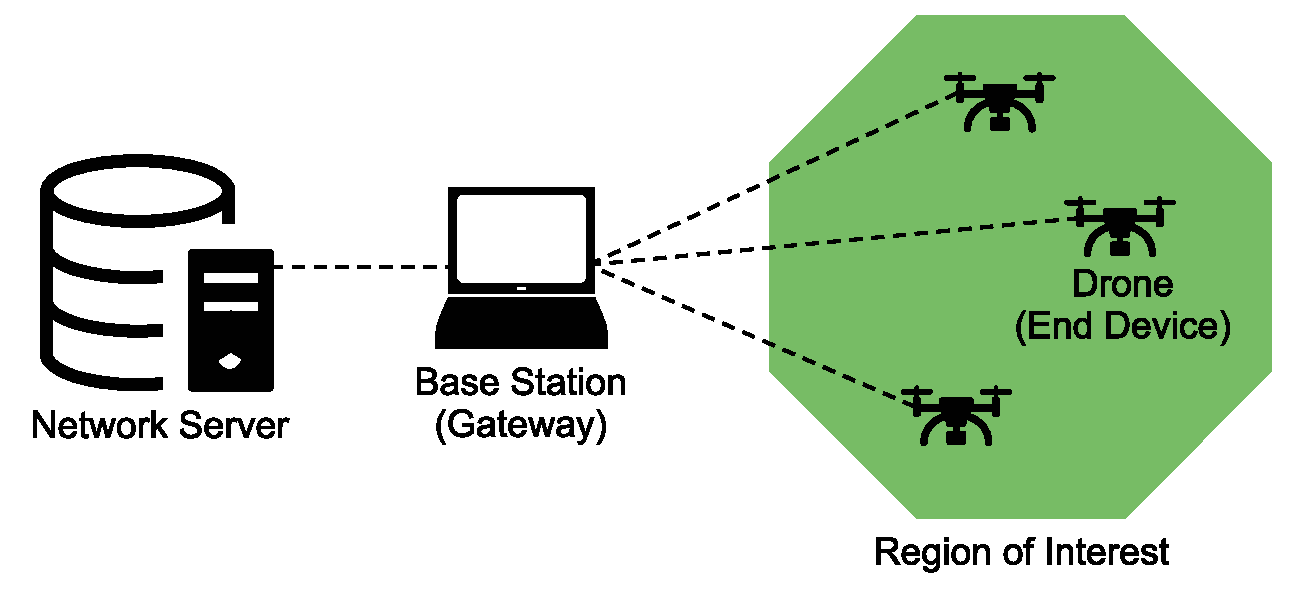
\includegraphics[width=0.7\linewidth]{figs/Jihwan/Network Diagram of LoRa.eps}
    \caption[LoRaWAN Network Diagram for Extra-UAV Communication]
    {\gls{lorawan} network diagram for extra-\gls{UAV} communication. More base stations, \gls{roi}s and drones can be connected to the network server as necessary.}
    \label{fig:euc_network_diagram}
\end{figure}

When generating the path plan of the drones in the mission planning framework (Section~\ref{sec:msp}), a network simulation will be conducted to ensure signal stability throughout the entire duration of the mission. If the drone paths travel too far from the base station for a stable extra-\gls{UAV} communication to be maintained, the operator will be warned and advised to install another base station at a suitable location. 
 
\subsubsection{Simulation using ns-3}

To simulate the stability of \gls{lorawan} during a mission, ns-3\footnote{\url{https://www.nsnam.org/}} discrete-event network simulator is used. ns-3 is a free and open-source software (GNU GPLv2 license) which allows the developer to incorporate custom models to construct the simulation scenario. 

\paragraph{LoRaWAN Model} The model was created by \cite{magrin2017lora} to create \gls{lorawan} simulations by establishing connections between custom end devices, gateways and network servers. Currently, the model only supports class A end devices at 868\,MHz (\gls{ism} band for EU) so additional components will need to be developed for implementation. 

\paragraph{Mobility Model} The model enables nodes to have defined position and velocities on a Cartesian plane. The generated path plans of the drones can be input to accurately simulate the network performance at any part of the \gls{roi} during the mission. 
